\documentclass[../main.tex]{subfiles}
 
\begin{document}

The project now has the capability to decode YCbCr components of the first intra frame from raw H.264 bitstream,
which means the following functionalities have been implemented:

\begin{itemize}
\item Bitstream parsing
\item Intra prediction generation
\item Inverse quantization
\item Inverse transformation
\end{itemize}

Figure \ref{fig:output} shows the reference frame and decoded frame of test data Foreman QCIF.

\begin{figure} [ht]
\begin{center}
\begin{tabular}{c} %% tabular useful for creating an array of images 
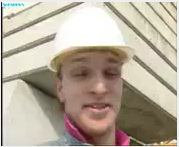
\includegraphics[height=5cm]{reference.png}

\includegraphics[height=5cm]{output.png}
\end{tabular}
\end{center}
\caption[output] 
{ \label{fig:output} Reference frame (left) and decoded frame (right)}
\end{figure} 

\end{document}